\documentclass[UTF8]{ctexart}
\usepackage[a4paper,left=3cm,right=3cm,top=2cm]{geometry}
\usepackage{amsmath}
\usepackage{enumitem}
\usepackage{float}
\usepackage{threeparttable}
\usepackage{caption}
\usepackage{multirow}
\usepackage{graphicx}

\setlength\lineskiplimit{5.25bp}
\setlength\lineskip{5.25bp}

\title{单摆法测量重力加速度——实验报告}
\author{崔士强 PB22151743}
\date{\today}

\bibliographystyle{plain}

\begin{document}

\maketitle
\section{实验目的}
利用单摆测量所在地的重力加速度.
\section{实验原理}
\noindent 本实验中满足以下条件:
\begin{enumerate}
    \item 细绳质量$\ll$小球质量
    \item 小球直径$\ll$细绳长度
    \item 摆角$\theta <5^\circ$
\end{enumerate}
因此有近似公式
\[T=2\pi\sqrt{\frac{l}{g}}\]
测出摆长及周期即可得出重力加速度.
\section{实验仪器}
本实验中用到的仪器有:钢卷尺,电子秒表,单摆(带标尺,平面镜,摆线长度可调),所使用仪器的最大允差以及估计误差如下表所示
\begin{table}[H]\centering
    \begin{tabular}{cccc}
        \hline\hline
        \multicolumn{2}{c}{钢卷尺}&\multicolumn{2}{c}{秒表}\\
        $\Delta_\text{仪}/cm$ & $\Delta_\text{估}/cm$ & $\Delta_\text{仪}/s$ & $\Delta_\text{估}/s$ \\
        \hline
        0.2&0.05&0.01&0.2\\
        \hline\hline
    \end{tabular}
    \caption{仪器的最大允差及估计误差}
\end{table}
\clearpage
\section{实验数据及处理}
实验数据见下表,原始数据记录照片见文档尾.
\begin{table}[H]\centering
    \begin{tabular}{ccc}
        \hline\hline
        次数 & 摆长 $l/cm$ & 总时间 $t/s$ \\
        \hline
        1 & 70.00 & 84.12 \\
        2 & 70.05 & 83.91 \\
        3 & 70.03 & 84.09 \\
        4 & 70.20 & 84.03 \\
        5 & 70.05 & 84.13 \\
        \hline\hline
    \end{tabular}%
    \qquad
    ($n=50$)
    \caption{实验数据}
\end{table}
\noindent 摆线长度l的平均值
$$
\overline{l}=\frac{1}{n}\sum_{i=1}^{n}l_i=\frac{70+70.05+70.03+70.2+70.05}{5}\,\mathrm{cm}=70.066\,\mathrm{cm}
$$
摆长l的标准差
$$
\begin{small}
\begin{aligned}
\sigma_{l}&=\sqrt{\frac{1}{n-1}\sum_{i=1}^n\left(l_i-\overline{l}\right)^2}\\
&=\sqrt{\frac{(70-70.066)^2+(70.05-70.066)^2+(70.03-70.066)^2+(70.2-70.066)^2+(70.05-70.066)^2}{5-1}}\,\mathrm{cm}\\
&=0.077653\,\mathrm{cm}
\end{aligned}
\end{small}
$$
摆长l的B类不确定度
$$
\Delta_{B,l}=\sqrt{\Delta_\text{仪}^2+\Delta_\text{估}^2}=\sqrt{0.2^2+0.05^2}\,\mathrm{cm}=0.20616\,\mathrm{cm}
$$
摆长l的展伸不确定度
$$
\begin{aligned}
U_{l,P}&=\sqrt{\left(t_P\frac{\sigma_{l}}{\sqrt{n}}\right)^2+\left(k_P\frac{\Delta_{B,l}}{C}\right)^2}\\
&=\sqrt{\left(2.78\times\frac{0.077653}{\sqrt{5}}\right)^2+\left(1.96\times\frac{0.20616}{3}\right)^2}\,\mathrm{cm}\\
&=0.16571\,\mathrm{cm},P=0.95
\end{aligned}
$$

\noindent 周期T的平均值
$$
\overline{T}=\frac{1}{n}\sum_{i=1}^{n}T_i=\frac{1.6824+1.6782+1.6818+1.6806+1.6826}{5}\,\mathrm{s}=1.6811\,\mathrm{s}
$$
周期T的标准差
$$
\begin{small}
\begin{aligned}
\sigma_{T}&=\sqrt{\frac{1}{n-1}\sum_{i=1}^n\left(T_i-\overline{T}\right)^2}\\
&=\sqrt{\frac{(1.6824-1.6811)^2+(1.6782-1.6811)^2+(1.6818-1.6811)^2+(1.6806-1.6811)^2+(1.6826-1.6811)^2}{5-1}}\,\mathrm{s}\\
&=0.0018089\,\mathrm{s}
\end{aligned}
\end{small}
$$
周期T的B类不确定度
$$
\Delta_{B,T}=\sqrt{\left(\frac{\Delta_\text{仪}}{n}\right)^2+\left(\frac{\Delta_\text{估}}{n}\right)^2}=\sqrt{0.0002^2+0.004^2}\,\mathrm{s}=0.004005\,\mathrm{s}
$$
周期T的展伸不确定度
$$
\begin{aligned}
U_{T,P}&=\sqrt{\left(t_P\frac{\sigma_{T}}{\sqrt{n}}\right)^2+\left(k_P\frac{\Delta_{B,T}}{C}\right)^2}\\
&=\sqrt{\left(2.78\times\frac{0.0018089}{\sqrt{5}}\right)^2+\left(1.96\times\frac{0.004005}{3}\right)^2}\,\mathrm{s}\\
&=3.4502 \times 10^{-3}\,\mathrm{s},P=0.95
\end{aligned}
$$

\noindent 重力加速度g
$$
g=\frac{4 \pi^{2} L}{T^{2}}=\frac{4\times \pi^2\times 0.70066}{1.6811^2}\,\mathrm{m/s^2}=9.7874\,\mathrm{m/s^2}
$$
重力加速度g的延伸不确定度
$$
\begin{aligned}
U_{g,P}&=\sqrt{\left(\frac{\partial g}{\partial l}U_{l,P}\right)^2+\left(\frac{\partial g}{\partial T}U_{T,P}\right)^2}\\
&=\sqrt{\left(\frac{4 \pi^{2}}{T^{2}}U_{l,P}\right)^2+\left(- \frac{8 \pi^{2} l}{T^{3}}U_{T,P}\right)^2}\\
&=\sqrt{\left(\frac{4\times \pi^2}{1.6811^2}\times 0.0016571\right)^2+\left(-\frac{8\times \pi^2\times 0.70066}{1.6811^3}\times 0.0034502\right)^2}\,\mathrm{m/s^2}\\
&=0.046367\,\mathrm{m/s^2},P=0.95
\end{aligned}
$$
重力加速度g最终结果
$$
g=\left(9.7874 \pm 0.05\right)\,\mathrm{m/s^2}
$$
\clearpage
\section{误差分析}
\noindent 本实验中
$$
\frac{\Delta g}{g}=\frac{2\times U_{g,P}}{g}\ \approx 0.0095
$$
满足$\Delta g/g<1\%$的要求,
实验误差的来源可能有以下几点\footnote{这里包括思考题的回答}:
\begin{enumerate}
    \item [1).] 摆长,总时间的测量存在误差
    \item [2).] 空气阻力对实验产生影响
\end{enumerate}
因此可作如下改进:
\begin{enumerate}
    \item [1).] 利用电脑软件对全过程的录像进行分析
    \item [2).] 适当减少周期数
\end{enumerate}
\section{原始数据记录}
\begin{figure}[h]
    \centering
    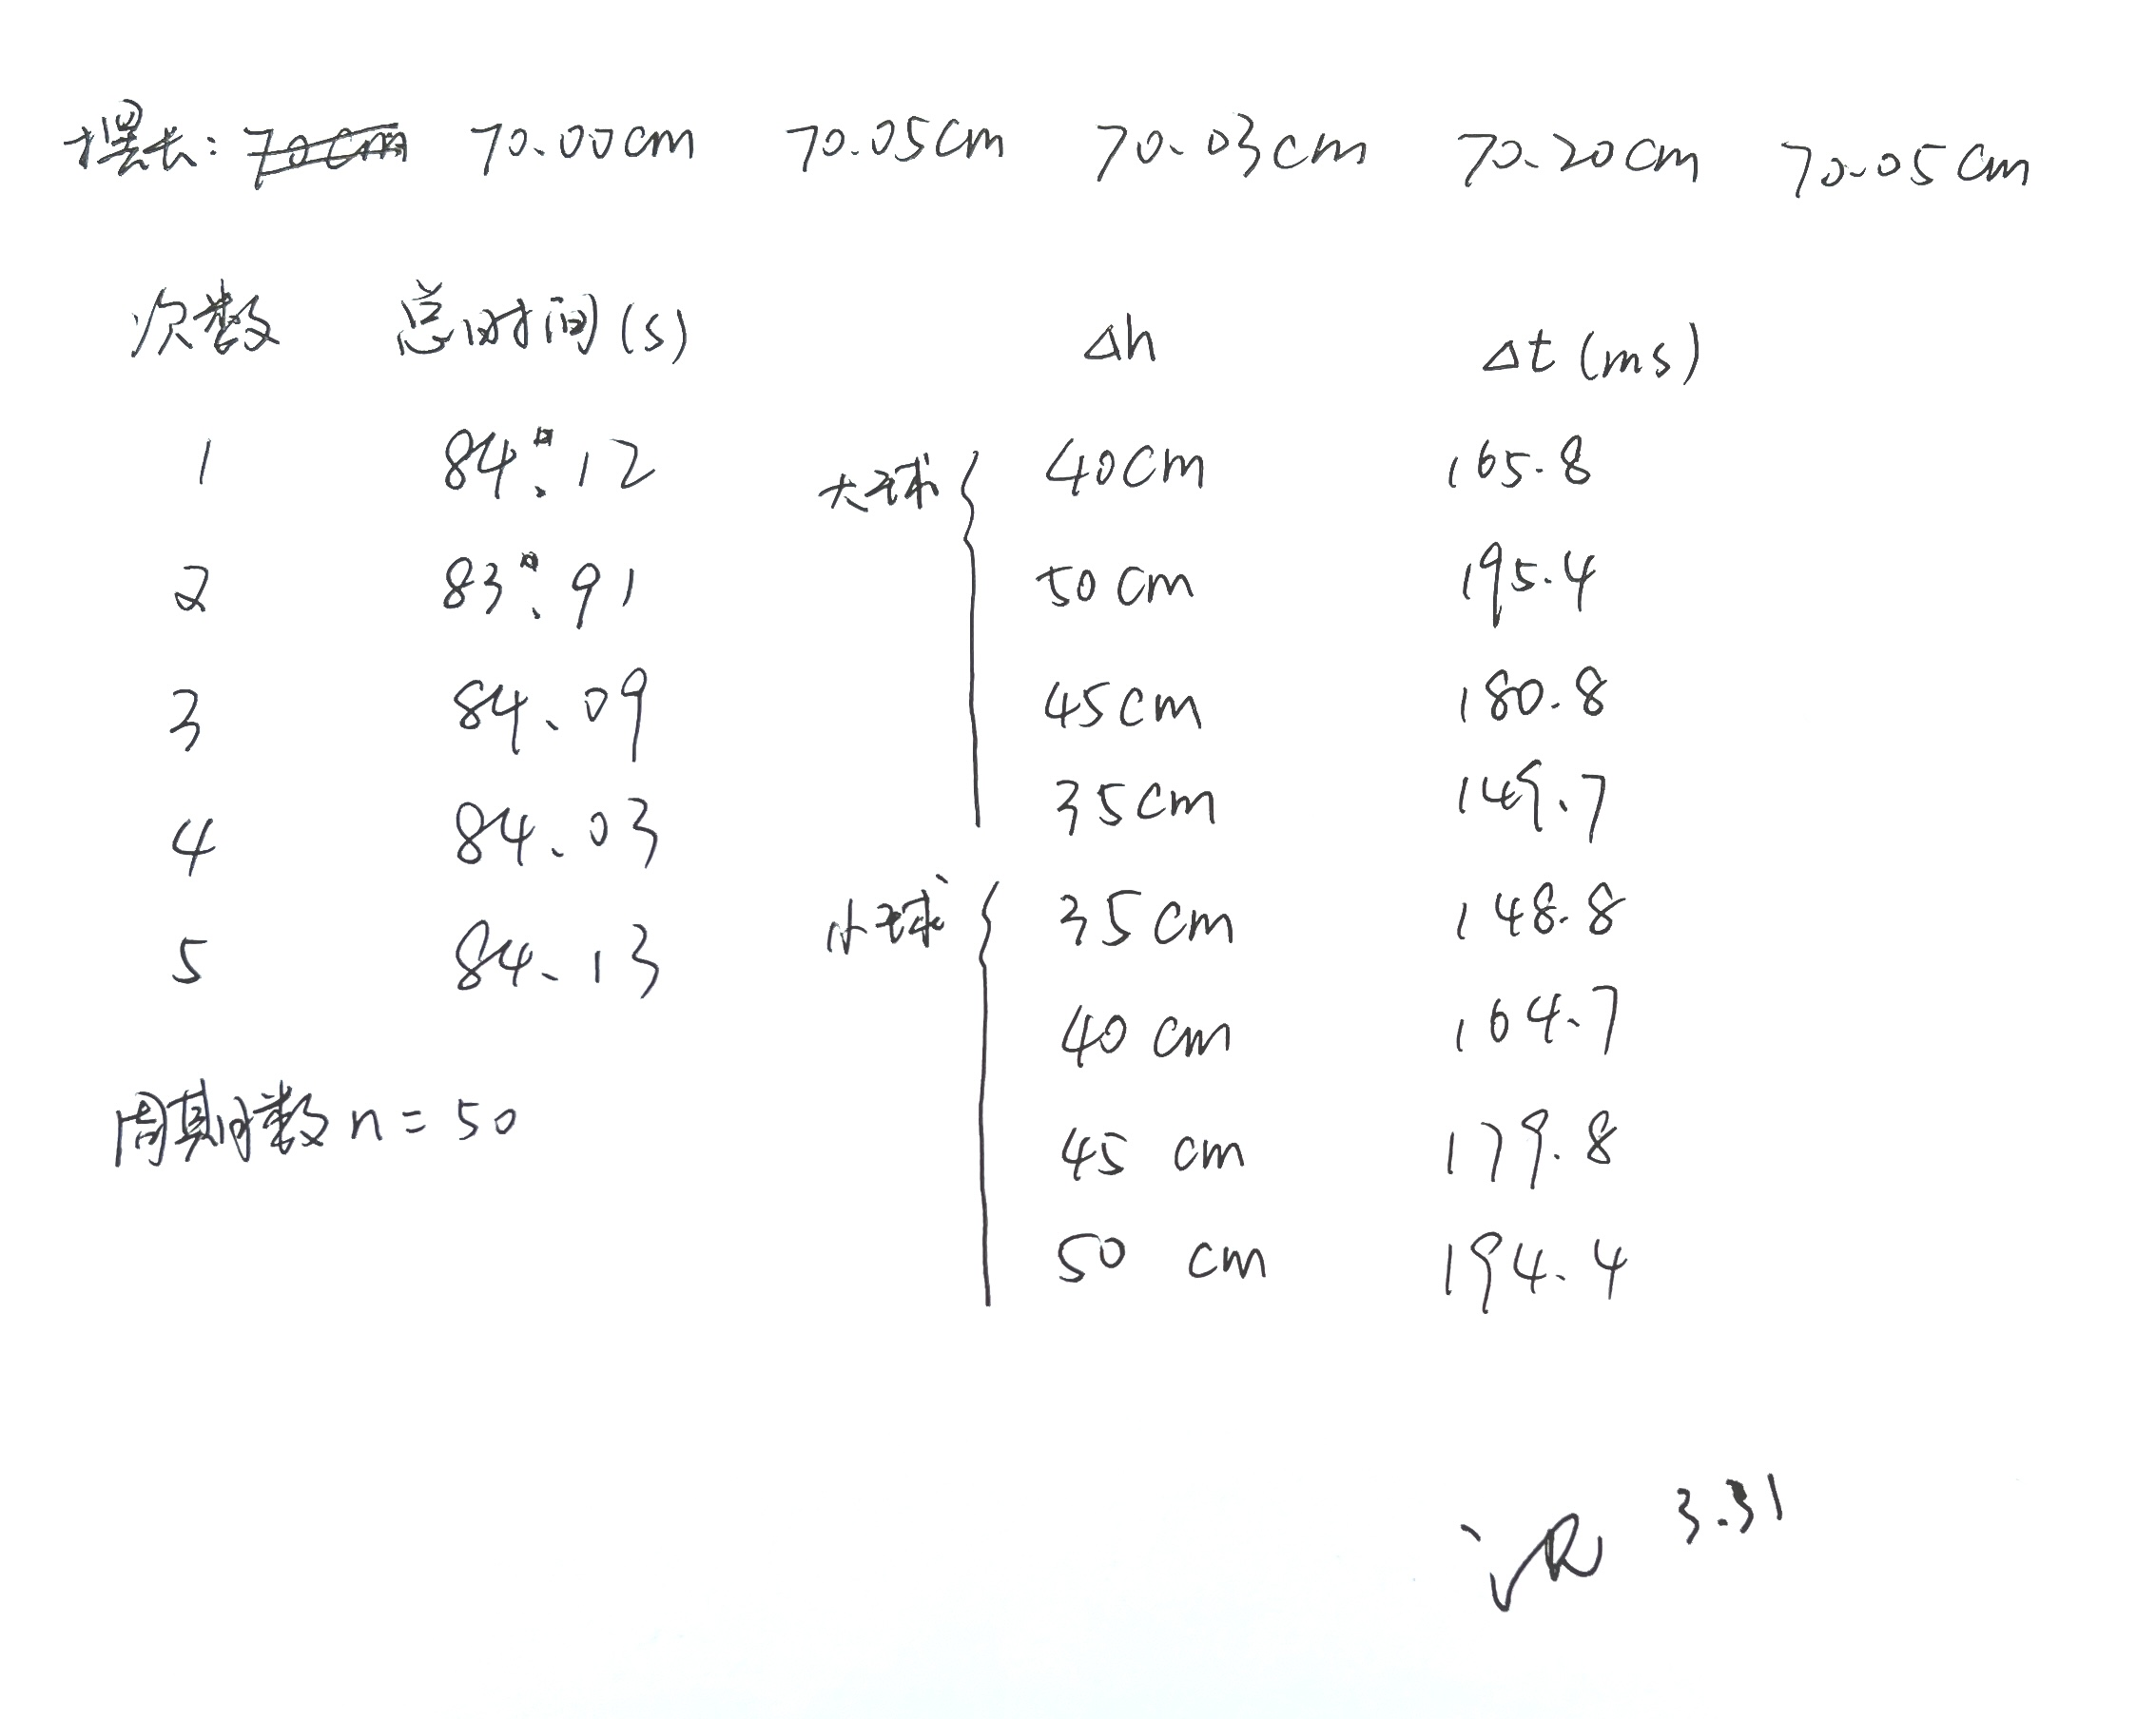
\includegraphics[scale=0.8]{data.png}
\end{figure}
\bibliography{math}

\end{document}